\subsubsection{Anatomy of ``Hello World!''}

Let's see more details of what the single line code we wrote is doing.

\ilcom{print()} is a build-in macro function that requests ImageJ to take the content within the parenthesis and print that out in the "Log" window. This content, which we genearlly call the \textit{argument} of the function, is an input value given to the function. The output of this function is the printed text in the Log window. Note that when a text is given as an argument, it must be surrounded by double quotes ("").

Where do we get information as such for other macro functions? The best reference for ImageJ macro functions is in the ImageJ web site
\footnote{\url{http://rsbweb.nih.gov/ij/developer/macro/functions.html}}. 
For example, you could find definition of \ilcom{print("")} function on the web site as quoted below:\\

\begin{indentCom}
\fbox{
\parbox[b][20em][c]{0.80\textwidth}{
\textbf{print(string)}\\
Outputs a string to the "Log" window. Numeric arguments are automatically converted to strings. 
The print() function accepts multiple arguments. For example, you can use print(x,y,width, height) 
instead of print(x+" "+y+" "+width+" "+height). 
If the first argument is a file handle returned by File.open(path), 
then the second is saved in the referred file (see SaveTextFileDemo).

Numeric expressions are automatically converted to strings using four decimal places, 
or use the \ilcom{d2s} function to specify the decimal places. 
For example, print(2/3) outputs "0.6667" but print(d2s(2/3,1)) outputs "0.7".

\dots
}
}
\end{indentCom}

As \ilcom{print} can do many things, its explanation is extraordinary long, but by carefully reading it, you will save time afterwards by the knowledge of wide spectrum of things that the \ilcom{print} function can do e.g. directly save text as a file.

Macro can be saved as a file.
In the editor, do \ijmenu{[File -> Save]}. Just save the file wherever you want in your file system. When you want to use the macro again, load the macro by \ijmenu{[File > Open]}.

\begin{indentexercise}
{1}
\item Add another line \texttt{"print("\textbackslash{}\textbackslash{}Clear");"} 
before the first line (below, code 1.51. don't forget the semi-colon at the end!). 
\item 
\begin{lstlisting}
//code 1.5
print("\\Clear");
print("Hello World!");


\end{lstlisting}
(code/code01_51.ijm)
Then test also another macro when you put the same line after "Hello World!". 
What happened? Any difference in the behavior? 
\item 
\begin{lstlisting}
//Code 1.76
print("Hello World!");
print("\\Clear");
\end{lstlisting}
(code/code01_76.ijm)
\item \textbf{Answer}: The first code prints "Hello World!", while the second code prints nothing. This is becaise \ilcom{print("\textbackslash{}\textbackslash{}Clear")} is a command that clears the Log window. In the first code, ``Hello World'' is printed after the window clearing, and in the second case the Log window is wiped out right after the printing of ``Hello World''. Effectively it looks like nothing has happened.  
\end{indentexercise}

\begin{indentexercise}
{2}
\item Try modifying the third line in code 1.51
and check that the modified text will be printed in the "Log" window. \\
\end{indentexercise}

\begin{indentexercise}
{3}
\item Multiple macros can exist in a single file. We call this \textbf{"macro sets"}. To distinguish each macro, each they each should have a specific name. For this, each macro should start with a special word ``macro'' followed by the name of the macro, and then a pair of curly braces to encapsulate its macro functions. See the code below.  


\begin{lstlisting}
macro "print_out" {
	print("Hello World!");
}

macro "print_out2" {
	print("Bye World!");
}

\end{lstlisting}
(code/code01_8.ijm)

Modify the code you already wrote in the script editor to wrap it inside a pair of macro bounds, the curly braces (\ilcom{\{\}}).  Then copy and paste the same under the first macro. 
The second macro should be modified to have a different name. In the example shown in fig.
\ref{fig_MacroSetInMenu}, the second macro is named "print\_out2".
\begin{figure}[htbp]
\begin{center}
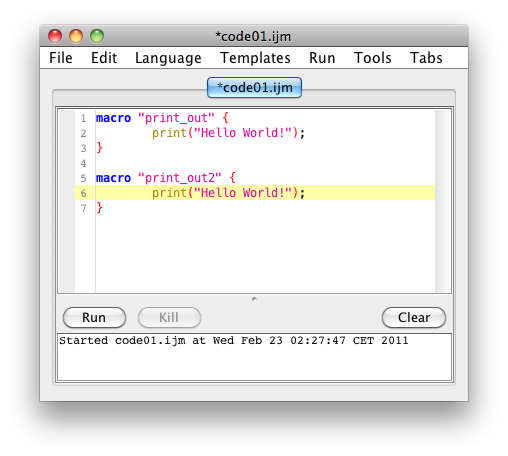
\includegraphics[scale=0.6]{fig/editor_MacroSet.png}
\caption{Macro Set} \label{fig_MacroSetInMenu}
\end{center}
\end{figure}
When macro is properly declared in this way, you could install the macro to have it as a menu item. To do so, in the editor menu select: 
\begin{indentFiji}
[Run -> Install Macro]).
\end{indentFiji}
In the main menu you should no be able to see the macro names under \ijmenu{[Plugins > Macros > ]}.

\begin{figure}[htbp]
\begin{center}
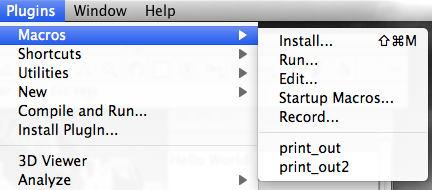
\includegraphics[scale=0.6]{fig/firstMacroSetInMenu.png}
\caption{Macro Now in ImageJ menu} \label{fig_MacroInMenu}
\end{center}
\end{figure}
\end{indentexercise}

\subsection{Variables and Strings}
Texts such as "Hello World!" can be represented by a variable 
\footnote{there is no declaration of types, such as number or string, in ImageJ macro.}.
Let's understand this by examining a short macro below.